\documentclass[10pt]{article}
\usepackage[utf8]{inputenc}
\usepackage[spanish]{babel}
\usepackage{amsfonts}
\usepackage{amsmath}
\usepackage{geometry}
\usepackage{graphicx}
\usepackage{caption}
\usepackage{subcaption}
 \usepackage{float}
\geometry{letterpaper, margin=1.5in}
\usepackage[linesnumbered,lined,boxruled,spanish,onelanguage]{algorithm2e}
\author{José Miguel Saavedra Aguilar}
\title{Tarea 01. Graficador de funciones}
\begin{document}
\maketitle
\begin{abstract}
En esta tarea se presenta un graficador de funciones reales en un intervalo $\left[ a,b \right] \subset \mathbb{R}$. Dicho graficador fue programado en Python utilizando la librería gráfica \texttt{Graphics.py} de John Zelle. Con esta librería, podemos graficar puntos, lineas, texto, y figuras geométricas básicas. El graficador funciona para funciones definidas para arreglos numéricos de \texttt{Numpy}, incluye un marco, malla, ejes coordenados y zoom sobre la función.\\
Así mismo, se estudian los detalles de la construcción estética del graficador, como es la malla, los ejes coordenados y la gráfica por sí misma. Finalmente, se hace una muestra del funcionamiento del graficador utilizando múltiples funciones evaluadas en distintos intervalos, lo que nos permite estudiar la función a detalle.
\end{abstract}
\section{Introducción}
La librería gráfica de Python \texttt{Graphics.py} fue creada por John Zelle para su libro \cite{Zelle2004} para trabajar con gráficos por computadora de forma orientada a objetos. En la versión 5, la más actual al día de hoy, podemos utilizar los siguientes objetos: Punto, linea, círculo, óvalo, rectángulo, polígono, texto e imágenes. La función principal de \texttt{Graphics.py} es \texttt{GraphWin(título, ancho, alto)}, que crea la ventana gráfica \texttt{título} de tamaño \texttt{ancho} $\times$ \texttt{alto}.
\section{Metodología}
Una vez que conocemos la librería gráfica, queda utilizarla para graficar una función $f:\mathbb{R}\mapsto\mathbb{R}$ en el intervalo $\left[a,b\right]$.\\
Para esto, iniciamos con un vector de $n$ puntos equiespaciados entre $a$ y $b$, que llamaremos $x_i$ para $i=1,...,n$. Así mismo, llamamos $y_i=f(x_i)$ a la función $f$ evaluada en $x_i$. Para evitar los errores numéricos con $x\approx x$ tales que $f$ no está definida en $x$, en el caso que $\left|y_i\right|>y_{max}$, no se tomará en cuenta este punto para el resto de los cálculos ni para graficar.\\
Ahora que tenemos todos los puntos de la gráfica, debemos reescalarlos para que sean visibles en la gráfica. En el graficador, se introduce el ancho $P_x$ y alto $P_y$, en pixeles, de la gráfica, así como si se desea un marco alrededor de ésta. El marco es de $w_{marco}=50$ px, pero es posible modificarlo a cualquier valor positivo. En caso de no desear marco, se toma como un marco de valor $w_{marco}=0$. Así, la ventana gráfica tendrá $P_y+2w_{marco}$ px de alto y $P_x+2w_{marco}$ px de ancho. Si llamamos $y_{max}, y_{min}$ al máximo y mínimo valor de todas las $y_i$ respectivamente, definimos las siguientes cantidades:
\begin{align*}
d_y&:=y_{max}-y_{min}\\
m_y&:=-\frac{P_y}{d_y}\\
b_y&:=w_{marco}-y_{max}m_y\\
d_x&:=b-a\\
m_x&:=\frac{P_x}{d_x}\\
b_x&:=w_{marco}-am_x
\end{align*}
Así, si tomamos $\hat{x}_i:=m_xx_i+b_x$, $\hat{y}_i:=m_yy_i+b_y$, tenemos
\begin{align*}
\hat{x}_1&=w_{marco}\\
\hat{x}_n&=P_x+w_{marco}\\
\min\limits_{i=1,...,n}\hat{y}_i&=w_{marco}\\
\max\limits_{i=1,...,n}\hat{y}_i&=P_y+w_{marco}
\end{align*}
Es decir, $\hat{x}_i,\hat{y}_i$ es un reescalamiento de la gráfica al tamaño, en pixeles, de la ventana. Los siguientes apartados son enteramente opcionales, pero dan una mejor apariencia a la gráfica.\\
El primero de estos es la malla sobre $x,y$. Pintarla es muy sencilla, pues son líneas rectas, sin embargo, la dificultad, si es que podemos llamarla así, es el intervalo de la malla. Una primera interpretación puede ser tomarla cada cierto intervalo, sin embargo esto puede resultar contraproducente con ciertas funciones, pues la escala de este intervalo no coincide con la escala de la gráfica. Otra opción es tomar un número fijo de intervalos a lo largo de la gráfico, sin embargo resta utilidad a la malla y es puramente estético. La forma en que se tomarán los intervalos de la gráfica es calculando la escala de la gráfica.
\begin{align*}
c_x&:=\left\lceil{\log_{10}\left(\frac{d_x}{2}\right)}\right\rceil -1\\
c_y&:=\left\lceil{\log_{10}\left(\frac{d_y}{2}\right)}\right\rceil -1\\
s_x&:=10^{c_x}\\
s_y&:=10^{c_y}
\end{align*}
Si colocamos la malla sobre los puntos que marcan $js_x$, $js_y$ para $j=-10,...,10$ tales que sean visibles, tendremos una malla de a lo más 21 cortes verticales y horizontales, que marca en escalas de magnitud de orden $10$, y que sirve como referencia para comparaciones. A la malla, se le agregan los ejes coordenados, cuando se pueden ver, y la escala de la gráfica. Esta escala está en los ejes coordenados cuando se muestran, o sobre el marco si no se muestran. El último elemento que añadimos a la gráfica antes de la función misma, es el título de la gráfica, especificado por el usuario.\\
Finalmente, para graficar la función, dibujamos una linea entre el punto $(\hat{x}_i,\hat{y}_i)$ y el punto $(\hat{x}_{i+1},\hat{y}_{i+1})$ para $i=1,...,n-1$ siempre que este punto se tome en cuenta para graficar.\\
Una vez que tenemos el graficador, resta hacer zoom dentro de la gráfica. Como se espera que el zoom pueda ser sobre cualquier punto de la gráfica, se creó una función que hace zoom de forma artificial. La forma en que lo logra es calculando el punto medio $c$ del intervalo $[a,b]$, $c=\frac{a+b}{2}$, y la amplitud $d_x$ del intervalo, $d_x=b-c$. Se procede a graficar $f$ en $[a,b]$. Una vez graficado, \texttt{Graphics.py} nos permite saber si se presiona una tecla, y cuál tecla se presionó. Con esta información, podemos hacer una ampliación (zoom 2.0x) de la gráfica, el graficador solicita un nuevo centro $c^{new}$, si es que se quiere cambiar, y reduce la amplitud a la mitad, es decir $d_x^{new}=\frac{d_x}{2}$. Así mismo, podemos hacer una reducción (zoom 0.5 x) de la gráfica, nuevamente se solicita un nuevo centro $c^{new}$, pero se aumenta la amplitud al doble, es decir $d_x^{new}=2d_x$. Una tercera opción es mover la gráfica sin hacer zoom, para esto se toma un nuevo centro $c^{new}$ y $d_x^{new}=d_x$. Posteriormente, se grafica $f$ en $[a^{new},b^{new}]$, donde
\begin{align*}
a^{new}&=c^{new}-d_x^{new}\\
b^{new}&=c^{new}+d_x^{new}
\end{align*}
\section{Resultados}
A continuación, se consideran los problemas de la tarea.
\subsection{Problema 1}
Así, tenemos un algoritmo graficador con el pseudocódigo \ref{alg:Graficador}, un graficador con zoom con el pseudocódigo \ref{alg:GraficadorZoom}.\\
\begin{algorithm}[htbp]
	\SetAlgoLined
	\KwIn{$f,a,b,n,P_x,P_y$, enmarcar, mostrar malla, mostrar ejes, título}
	\KwOut{keyInput}
	\leIf{enmarcar}{$w_{marco}\gets 50$}{$w_{marco}\gets 0$}
	\For{$i=1$ \KwTo $n$}{
		$x_i\gets\frac{(b-a)i+na-b}{n-1}$\;
		$y_i\gets f(x_i)$\;
		$graph_i\gets$ ¿$y_i$ está bien definido?
		}
	$y_{max}\gets\max(y_i)$; $y_{min}\gets\min(y_i)$\;
	$d_y\gets y_{max}-y_{min}$; $m_y\gets -\frac{P_y}{d_y}$; $b_y\gets w_{marco}-y_{max}m_y$\;
	$d_x\gets b-a$; $m_x\gets \frac{P_x}{d_x}$; $b_x\gets w_{marco}-am_x$\;
	$\hat{x}_i\gets m_xx_i+b_x$; $\hat{y}_i\gets m_yy_i+b_y$\;
	inicializarGráfico($P_x+2w_{marco},P_y+2w_{marco}$)\;
	\If{mostrar malla}{
		$c_x\gets \left\lceil{\log_{10}\left(\frac{d_x}{2}\right)}\right\rceil -1$; $s_x\gets 10^{c_x}$\;
		$c_y\gets \left\lceil{\log_{10}\left(\frac{d_y}{2}\right)}\right\rceil -1$; $s_y\gets 10^{c_y}$\;
		\For{$j=\left\lfloor{\frac{a}{s_x}}\right\rfloor+1$ \KwTo $\left\lceil{\frac{b}{s_x}}\right\rceil$}{
			Pintar línea de $(s_xm_xj+b_x,w_marco)$ a $(s_xm_xj+b_x,P_y+w_{marco})$\;
			}
		\For{$j=\left\lfloor{\frac{y_{min}}{s_y}}\right\rfloor +1$ \KwTo $\left\lceil{\frac{y_{max}}{s_y}}\right\rceil$}{
			Pintar línea de $(w_{marco},s_ym_yj+b_y)$ a $(P_x+w_{marco},s_ym_yj+b_y)$\;
			}
		}
	\lIf{enmarcar}{
		Pintar cuadro de $(w_{marco},w_{marco})$ a $(P_x+w_{marco},P_y+w_{marco})$
		}
	\If{mostrar ejes}{
		\eIf{$y_{min}y_{max}<0$}{
  			Pintar línea de $(w_{marco},b_y)$ a $(P_x+w_{marco},b_y)$\;
  			Escribir escala de $x$ debajo de la linea anterior\;
  			}{
  			Escribir escala de $x$ debajo del marco\;
  			}
  		\eIf{$ab<0$}{
  			Pintar línea de $(b_x,w_{marco})$ a $(b_x,P_y+w_{marco})$\;
  			Escribir escala de $y$ a la izquierda de la linea anterior\;
  			}{
  			Escribir escala de $y$ a la izquierda del marco\;
  			}
  		}
  	\lIf{título no es vacío}{
  		Escribir título en $\left(w_{marco}+\frac{P_x}{2},\frac{w_{marco}}{2}\right)$
  		}
  	\For{$i=1$ \KwTo $n-1$}{
  		\lIf{$graph_i$}{Pintar línea de $(\hat{x}_i,\hat{y}_i)$ a $(\hat{x}_{i+1},\hat{y}_{i+1})$}
  		}
  \caption{Graficador de $f$ en $[a,b]$}\label{alg:Graficador}
\end{algorithm}
\begin{algorithm}[htbp]
	\SetAlgoLined
	\KwIn{$f,a,b,n,P_x,P_y$, enmarcar, mostrar malla, mostrar ejes, título}
	\KwOut{}
	$c_x\gets \frac{a+b}{2}$\;
	$d_x\gets b-c_x$\;
	\While{True}{
		\texttt{Graficar}({$f,a,b,n,P_x,P_y$,enmarcar,mostrar malla,mostrar ejes,título})\;
		keyInput$\gets$Tecla presionada\;
		\Switch{keyInput}{
			\uCase{Escape}{
				\texttt{break}}
			\uCase{+}{
				$c_x\gets$\texttt{float}(Entrada de Usuario)\;
				$d_x\gets\frac{d_x}{2}$\;
				}
			\uCase{-}{
				$c_x\gets$\texttt{float}(Entrada de Usuario)\;
				$d_x\gets 2d_x$\;
				}
			\Case{Enter}{
				$c_x\gets$\texttt{float}(Entrada de Usuario)\;
				}
			}
			$a\gets c_x-d_x$\;
			$b\gets c_x+d_x$\;
		}
  \caption{Graficador con zoom}\label{alg:GraficadorZoom}
\end{algorithm}
Para utilizar el graficador, debemos definir una función que pueda ser evaluada en un arreglo de \texttt{NumPy}, por ejemplo:



\begin{verbatim}
def seno(x):
	y=np.sin(x)
	return y
\end{verbatim}

\noindent Nuestro graficador tiene la siguiente sintaxis:
\begin{center}
\texttt{Graficar($f$,$a$,$b$,$n$,$P_x$,$P_y$,enmarcar,showGrid,showAxis,Título)}
\end{center}
donde $f$ es la función definida previamente, $a$ y $b$ son los extremos del intervalo donde se graficará, $n$ es el número de puntos a evaluar dentro de $[a,b]$, $P_x$ y $P_y$ son el tamaño en pixeles de la ventana gráfica, \texttt{enmarcar},\texttt{showGrid} y \texttt{showAxis} son Booleanos que definen si se muestra el marco, si se muestra la malla y si se muestran los ejes respectivamente; \texttt{Título} es un string que contiene el título de la gráfica.\\
A continuación, se dará un ejemplo del uso del Graficador para graficar la función $f(x)=\sin(x)$ en el intervalo $[-5,5]$, iniciando con la llamada del Graficador:

\begin{verbatim}
Graficar(np.sin,-5,5,800,800,800,True,True,True,"f(x)=sin(x)")
\end{verbatim}

\begin{figure}[htbp]
    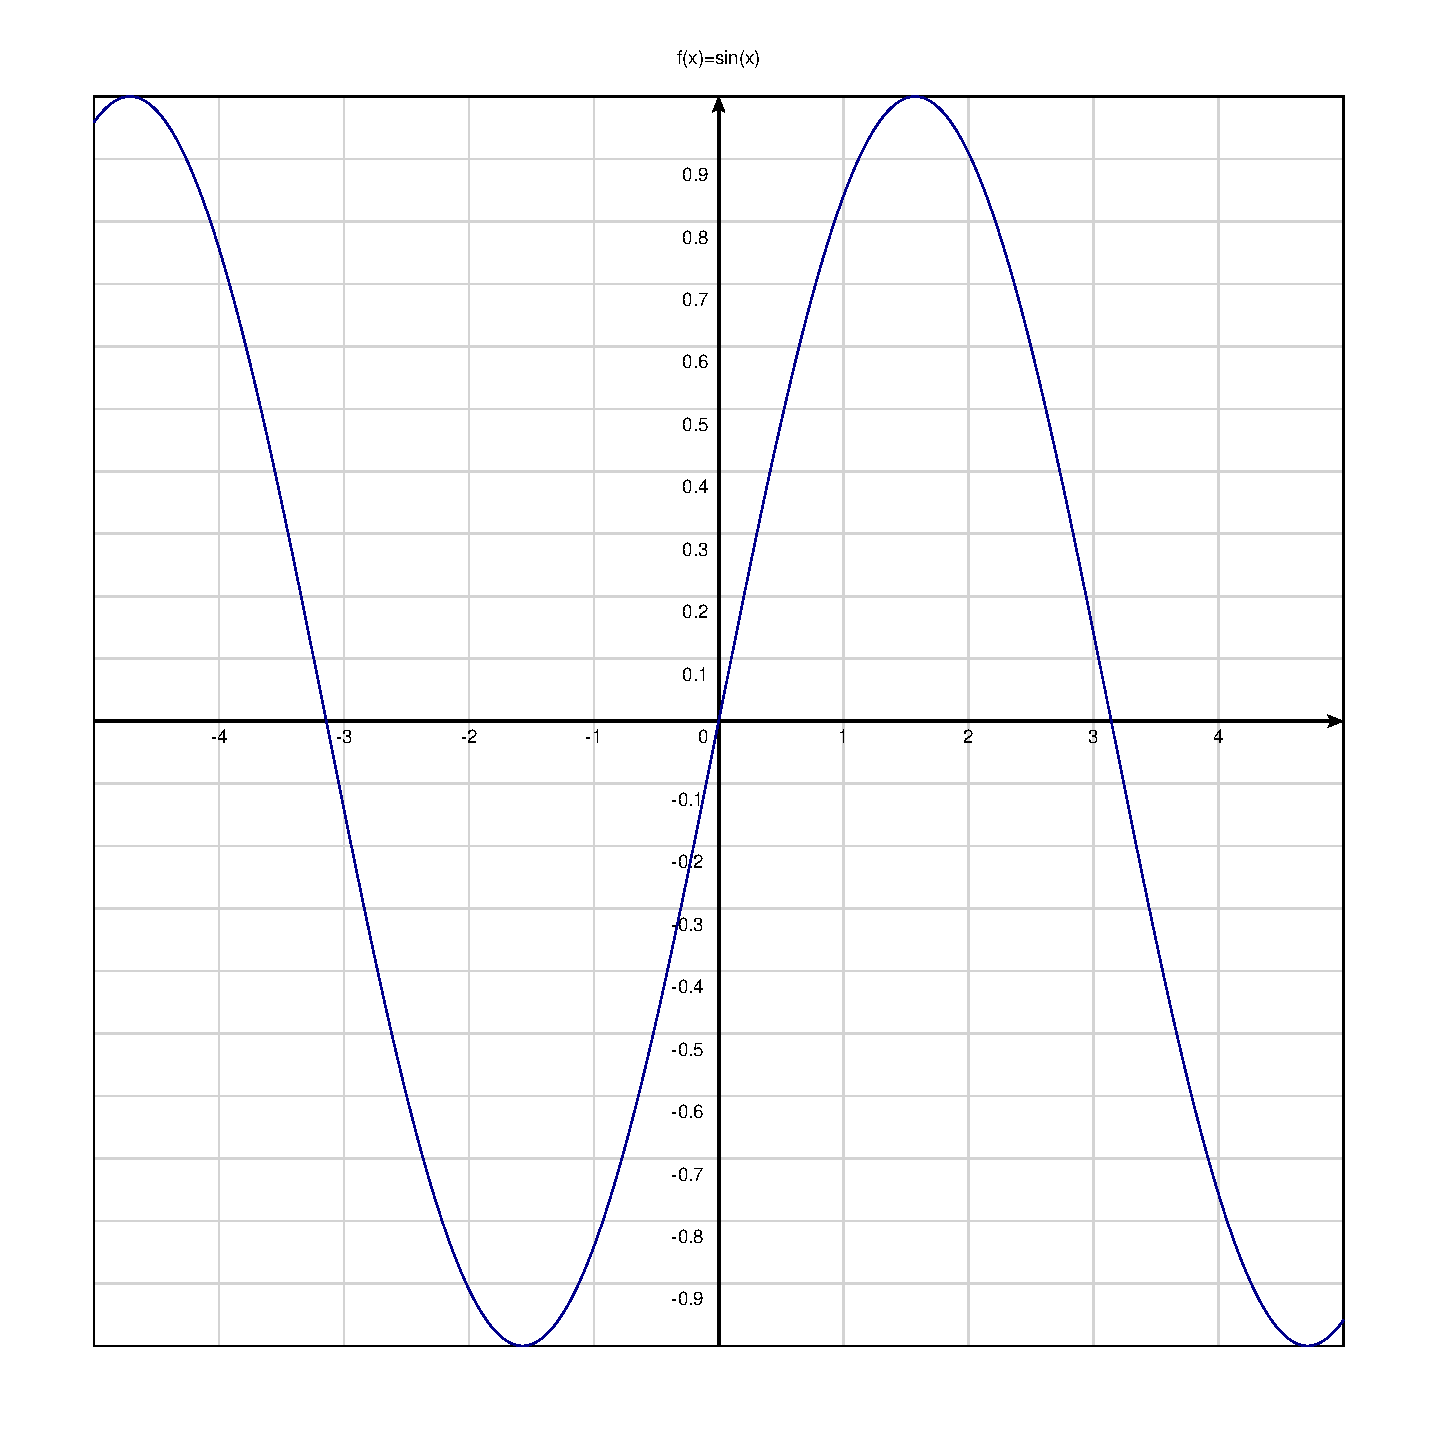
\includegraphics[scale=0.3]{figures/Seno.eps}
    \centering
    \caption{Función $y=\sin (x)$ graficada en $[-5,5]$}
    \label{im:Seno}
\end{figure}
\noindent La gráfica resultante se observa en la figura \ref{im:Seno}. Ahora, veamos el graficador con zoom, que como dijimos antes, lo manejamos como otra función que llama dentro al graficador. Este graficador con zoom es una función con la siguiente sintaxis:
\begin{center}
\texttt{GraficadorConZoom($f$,$a$,$b$,$n$,$P_x$,$P_y$,enmarcar,showGrid,showAxis,Título)}
\end{center}
Donde todos los argumentos son idénticos a los del graficador. por lo que está de más explicarlos. El funcionamiento de este algoritmo es más interactivo, como se puede ver en el pseudocódigo \ref{alg:GraficadorZoom}.
\newpage
\noindent Iniciamos llamando al Graficador con Zoom:

\begin{verbatim}
GraficadorConZoom(np.sin,-5,5,800,800,800,True,True,True,"f(x)=sin(x)")
\end{verbatim}

\noindent Esto nos mostrará una gráfica idéntica a la obtenida con el graficador, sin embargo, el programa nos arroja el siguiente mensaje en la consola:

\begin{verbatim}
Presiona + para acercar (2X), - para alejar (0.5X), Enter para mover
\end{verbatim}

\noindent Siguiendo las indicaciones de este mensaje, si hacemos clic en la gráfica, para asegurarnos estar trabajando ahí y no en otra ventana, y presionamos la tecla + en nuestro teclado, nos dará el siguiente mensaje:

\begin{verbatim}
Centro actual es 0.0
\end{verbatim}

\noindent Si se desea un nuevo centro sobre $x$, se ingresa. De lo contrario, se presiona Enter para mantener el centro actual.\\
Por ejemplo, si elegimos hacer un acercamiento y mantener el mismo centro sobre $x$. tendremos la gráfica mostrada en la figura \ref{im:Seno2x}.\\
Si, en cambio, se presiona - en el teclado con la ventana de la gráfica activa, la gráfica se aleja, como se ve en la figura \ref{im:Seno05x}.\\
Finalmente, si presionamos Enter para elegir un nuevo centro, lo hacemos de la siguiente forma:

\begin{verbatim}
Centro actual es 0.0
Introduce nuevo centro de x: 1.5707963268
\end{verbatim}

\noindent Lo que mueve el centro de la gráfica al punto $x=1.5707963268\approx\frac{\pi}{2}$, como se observa en la figura \ref{im:SenoCentrado}.
\begin{figure}[htbp]
    \centering
    \begin{subfigure}[b]{0.3\textwidth}
        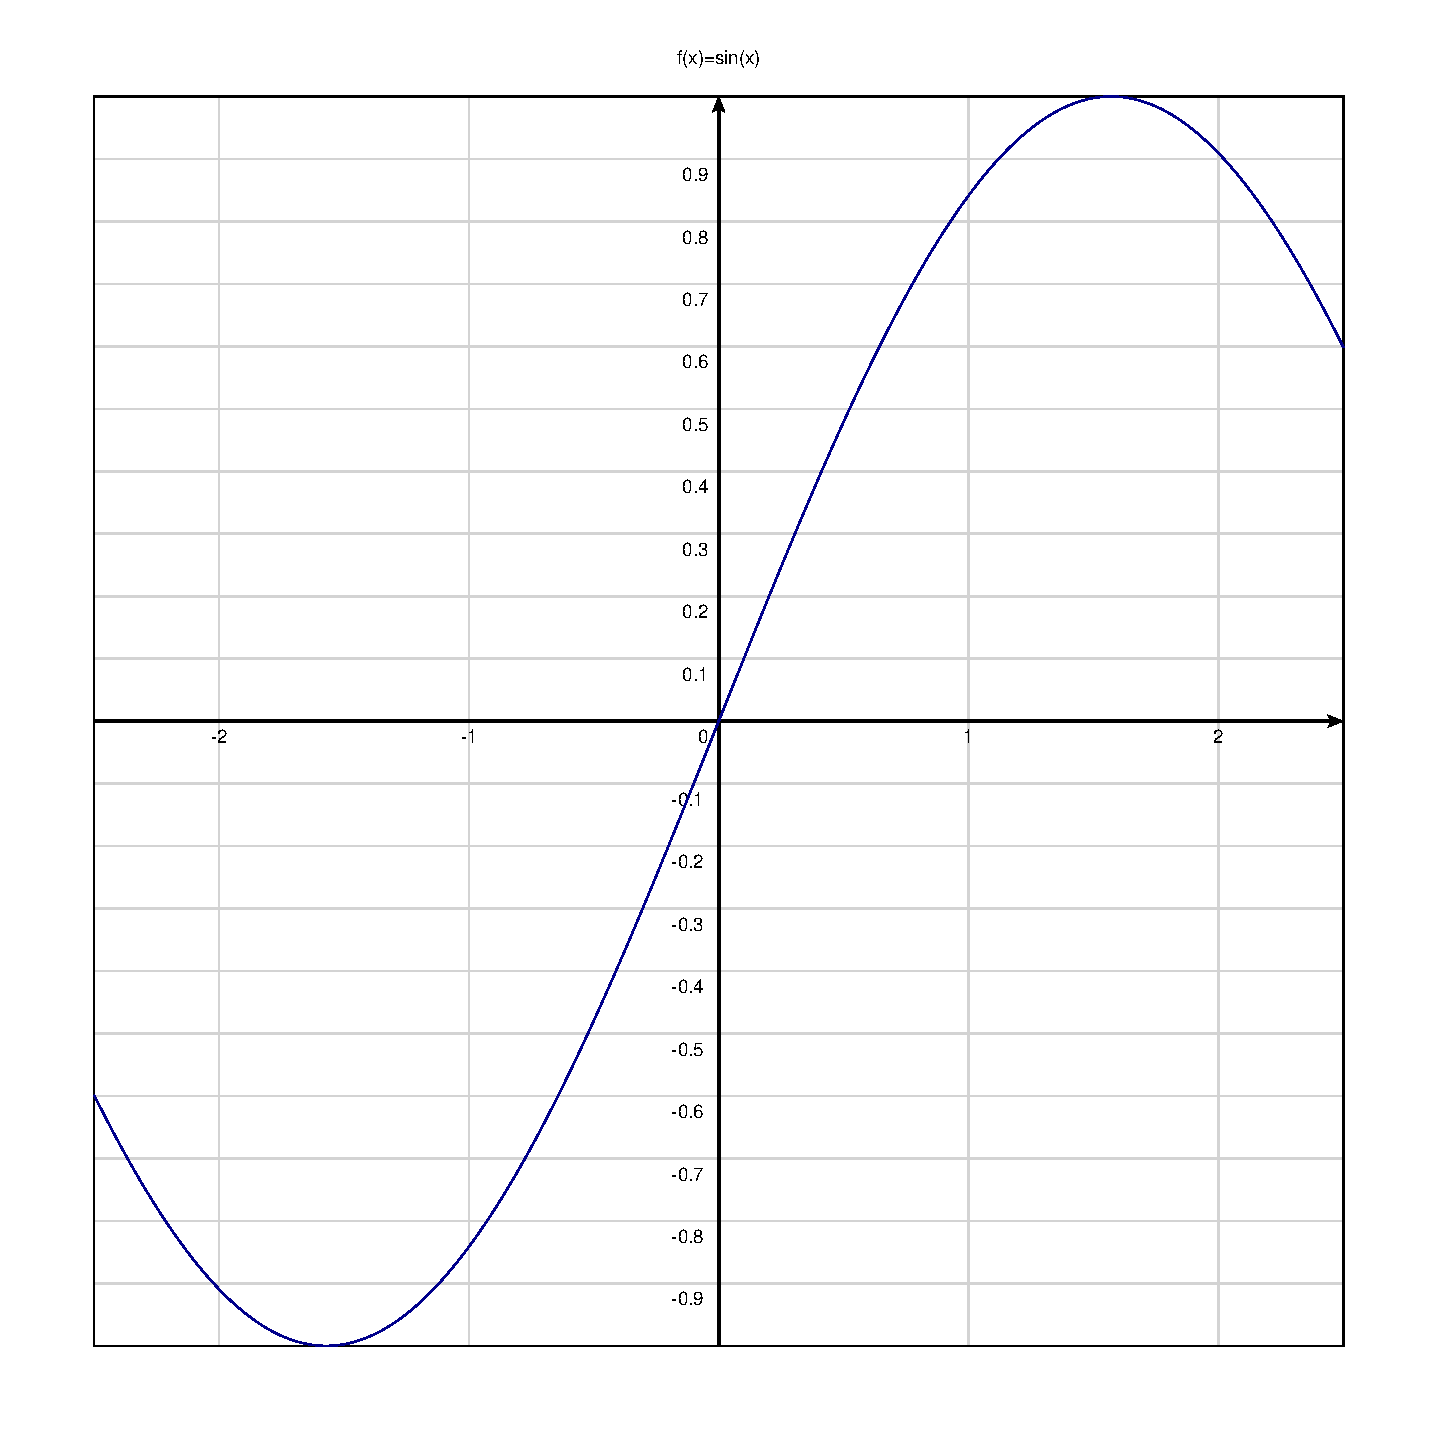
\includegraphics[width=\textwidth]{figures/Seno2x.eps}
        \centering
        \caption{Ejemplo de zoom 2.0x}
        \label{im:Seno2x}
    \end{subfigure}
    \hfill
    \begin{subfigure}[b]{0.3\textwidth}
        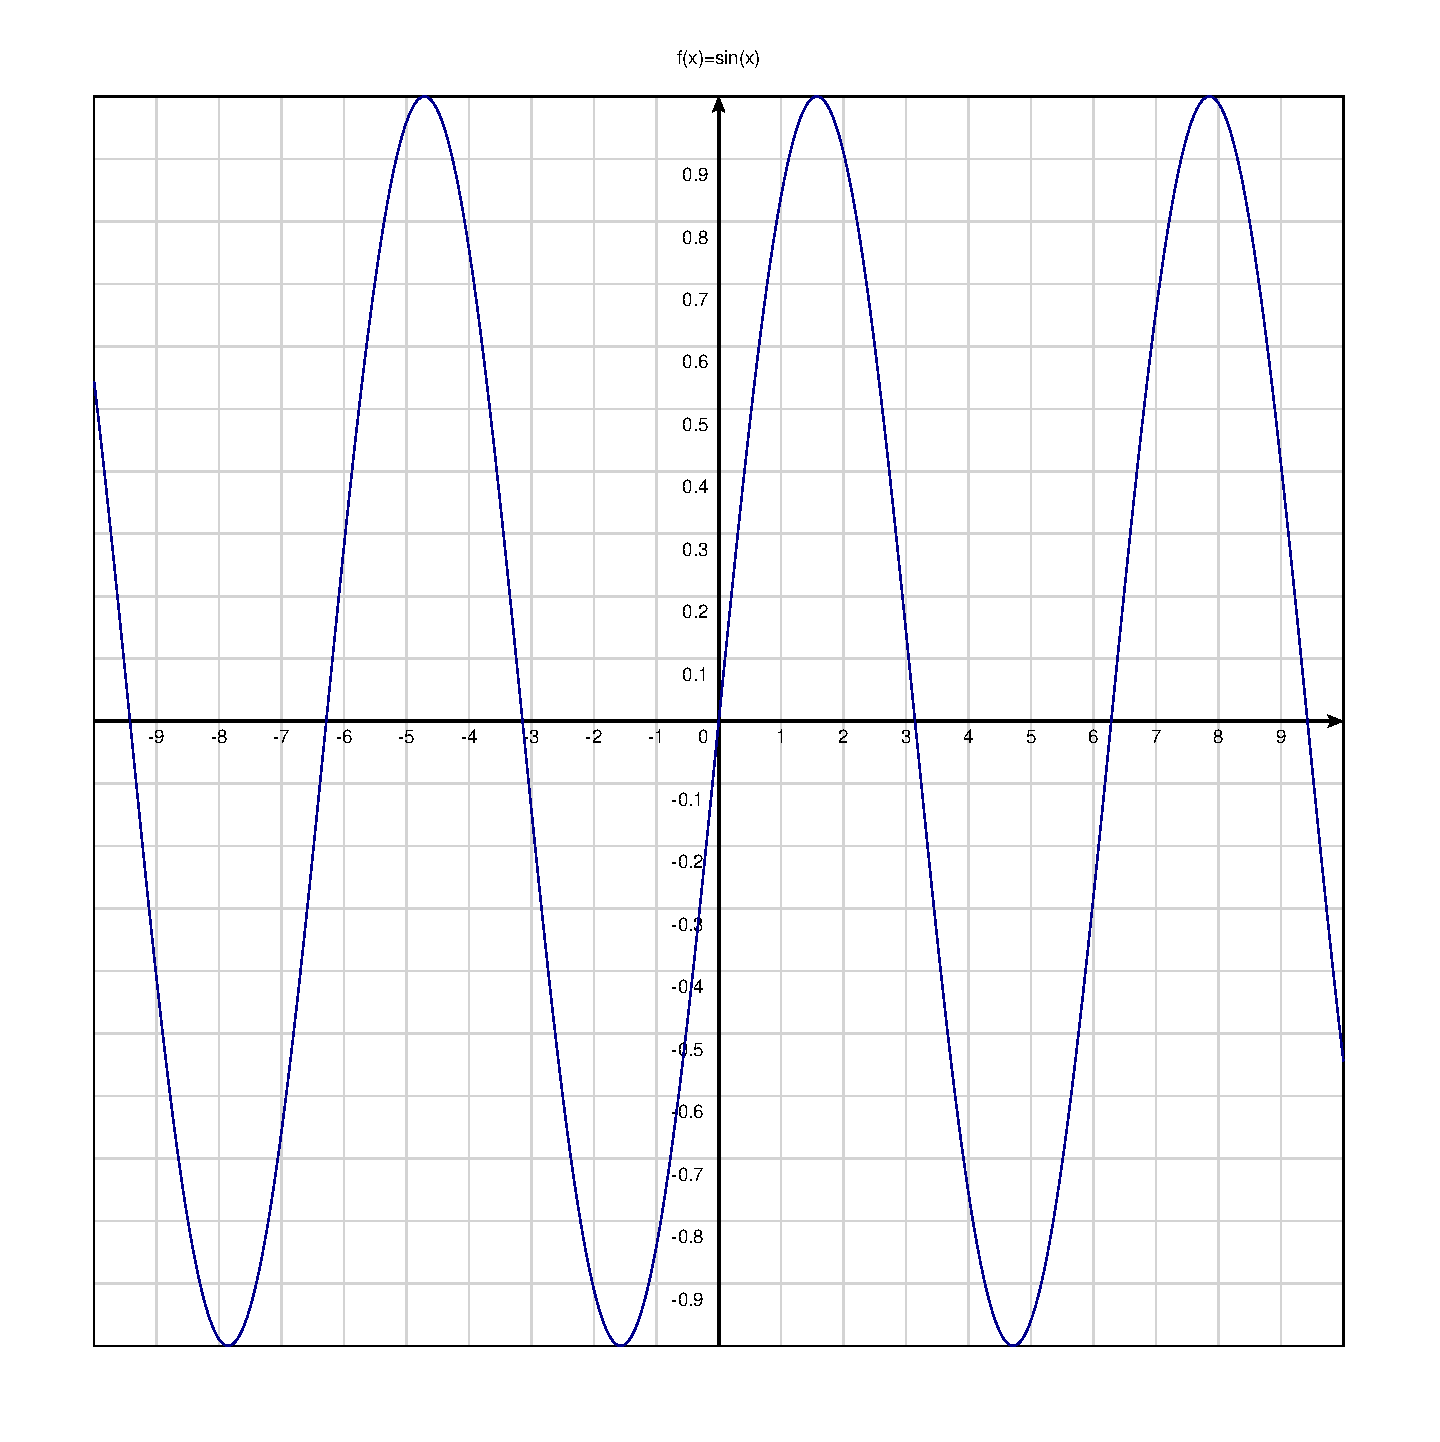
\includegraphics[width=\textwidth]{figures/Seno05x.eps}
        \centering
        \caption{Ejemplo de zoom 0.5x}
        \label{im:Seno05x}
    \end{subfigure}
    \hfill
    \begin{subfigure}[b]{0.3\textwidth}
        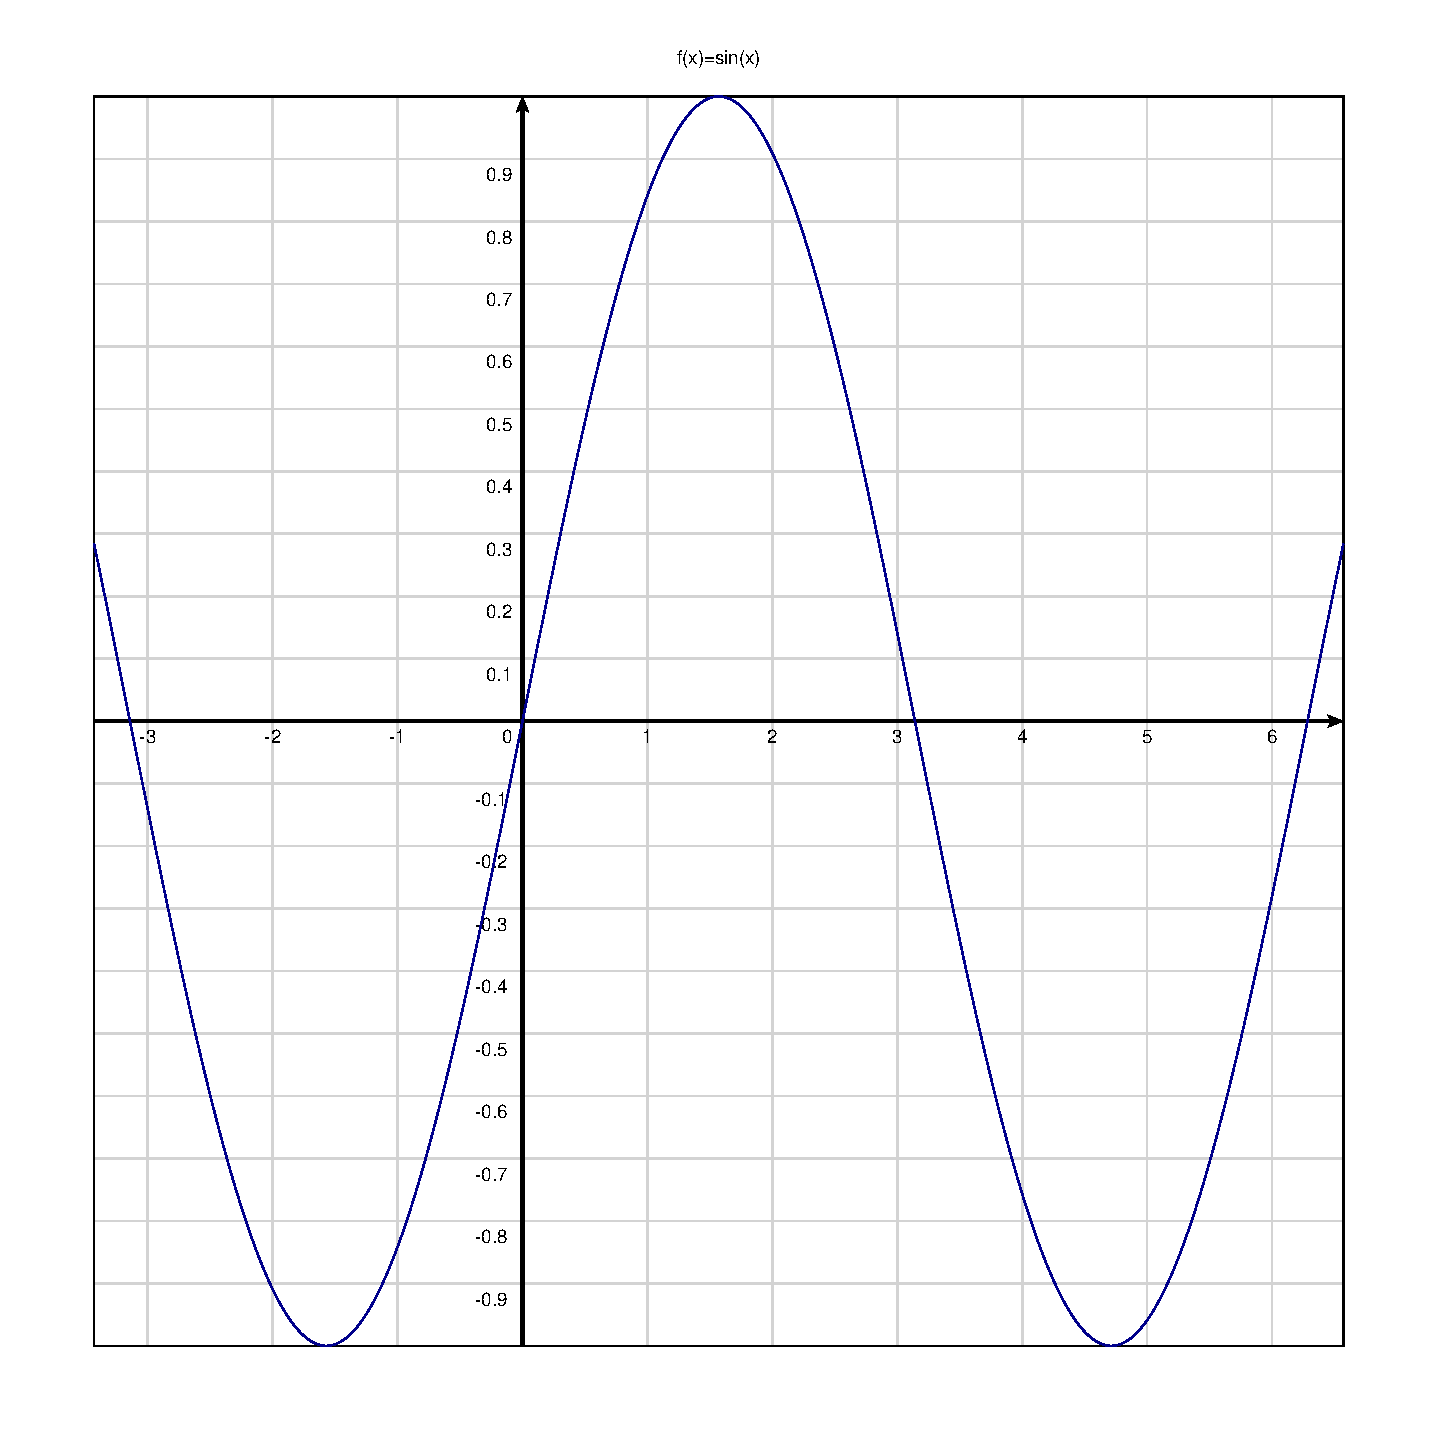
\includegraphics[width=\textwidth]{figures/SenoCentrado.eps}
        \centering
        \caption{Ejemplo de desplazamiento}
        \label{im:SenoCentrado}
    \end{subfigure}
    \caption{Ejemplos de uso del graficador con Zoom}
\end{figure}
\subsection{Problema 2}
La primera función a graficar es:
\begin{align}
f(x)&=x^3+x^2+1
\end{align}
Por lo que la definimos en Python y la graficamos:

\begin{verbatim}
def f(x):
    a=x**3+x**2+1
    return a
Graficar(f,-20,20,800,800,800,True,True,True,"f(x)=x³+x²+1")
\end{verbatim}

\noindent Ahora, la siguiente función está dada por:
\begin{align}
g(x)&=\sin (10x)
\end{align}
Igualmente, la definimos en Python y la graficamos:

\begin{verbatim}
def g(x):
    y=np.sin(10*x)
    return y
Graficar(g,-3,3,1600,800,800,True,True,True,"g(x)=sen(10x)")
\end{verbatim}

\noindent Obteniendo la gráfica de la figura \ref{im:graficaG}. Notamos que en este caso fue necesario hacer 1600 evaluaciones de la función debido a la naturaleza de la función, sin embargo esto no resulta en algún mayor problema. Finalmente, la última función está definida de la siguiente forma:
\begin{align}
h(x)&=\frac{1}{x+1}
\end{align}
A continuación, la definimos y graficamos

\begin{verbatim}
def h(x):
    y=1/(x+1)
    return y
Graficar(h,-20,20,800,800,800,True,True,True,"h(x)=1/(x+1)")
\end{verbatim}

\noindent Esto resulta en la gráfica mostrada en la figura \ref{im:graficaH}.
\begin{figure}[H]
    \begin{subfigure}[b]{0.3\textwidth}
        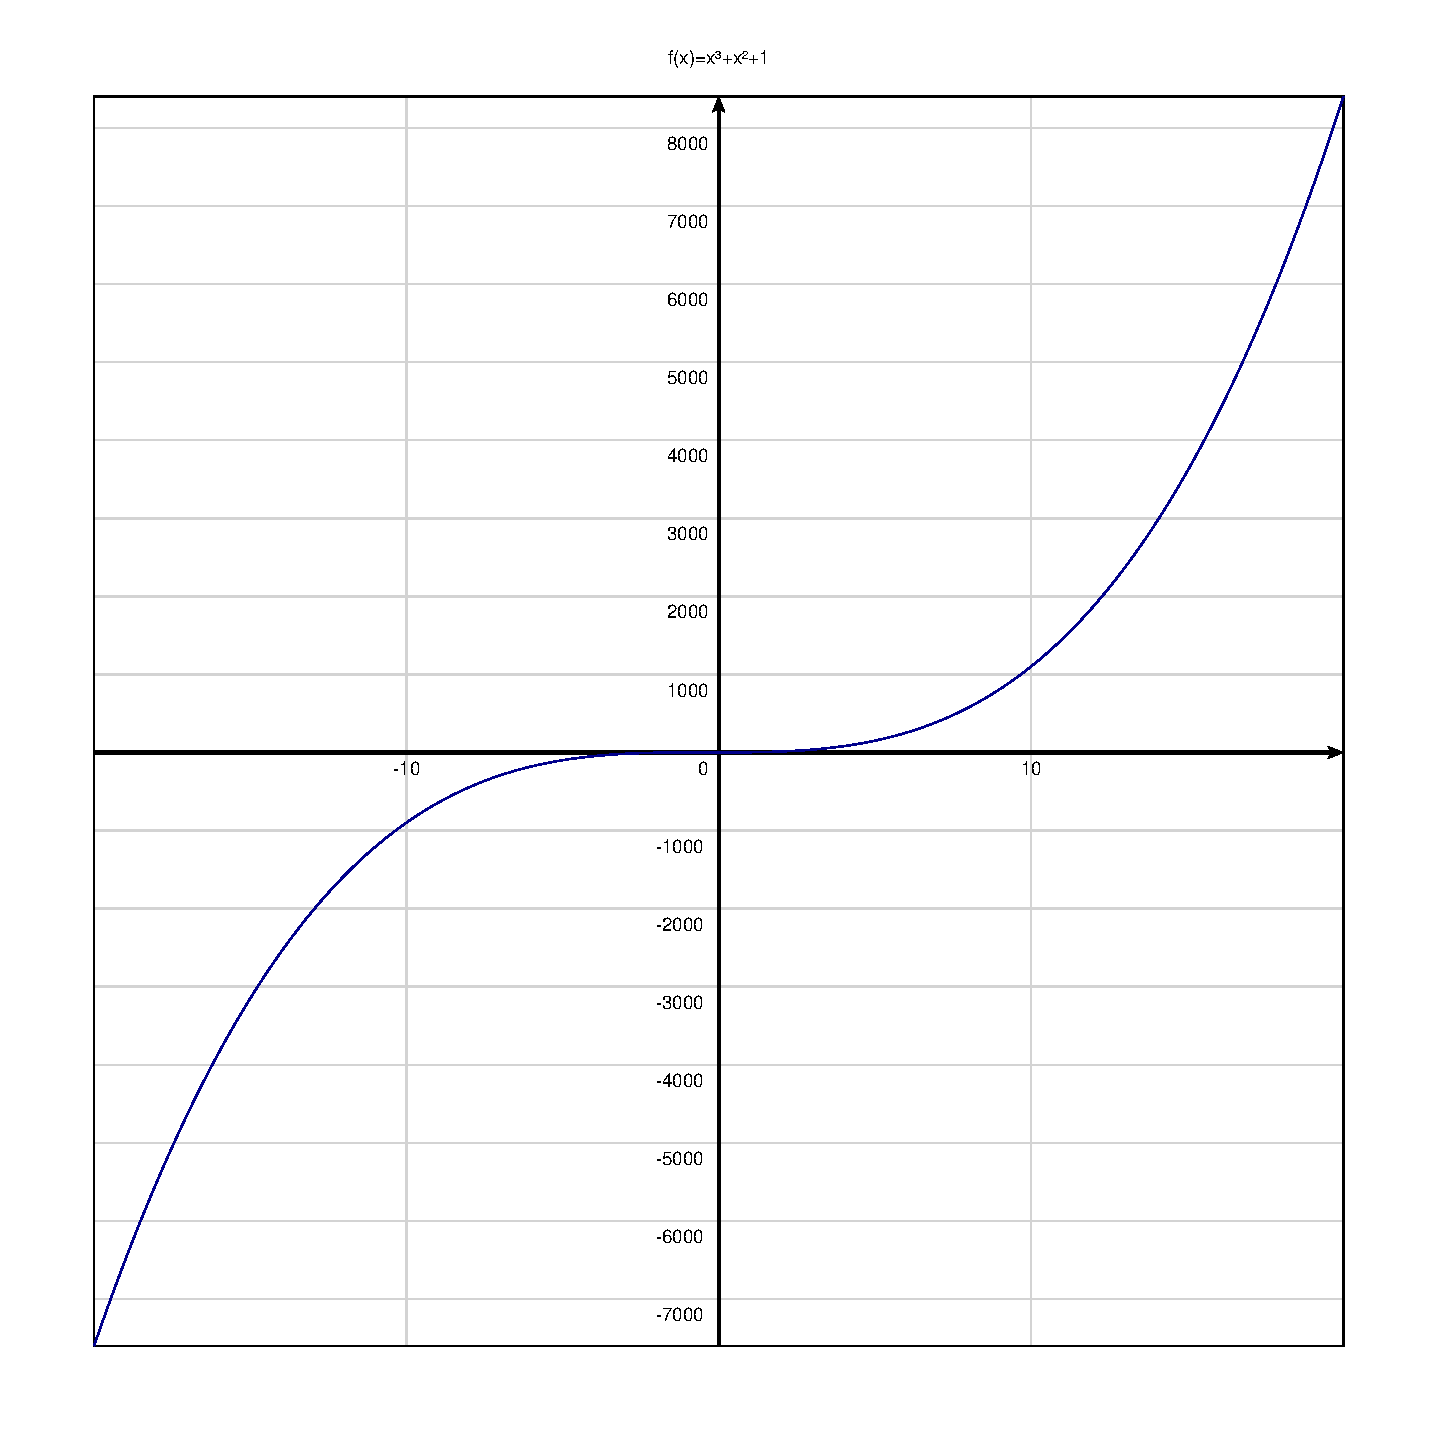
\includegraphics[width=\textwidth]{figures/graficaF.eps}
        \centering
        \caption{Gráfica de $f(x)$ evaluada en $[-20,20]$}
        \label{im:graficaF}
    \end{subfigure}
    \hfill
    \begin{subfigure}[b]{0.3\textwidth}
        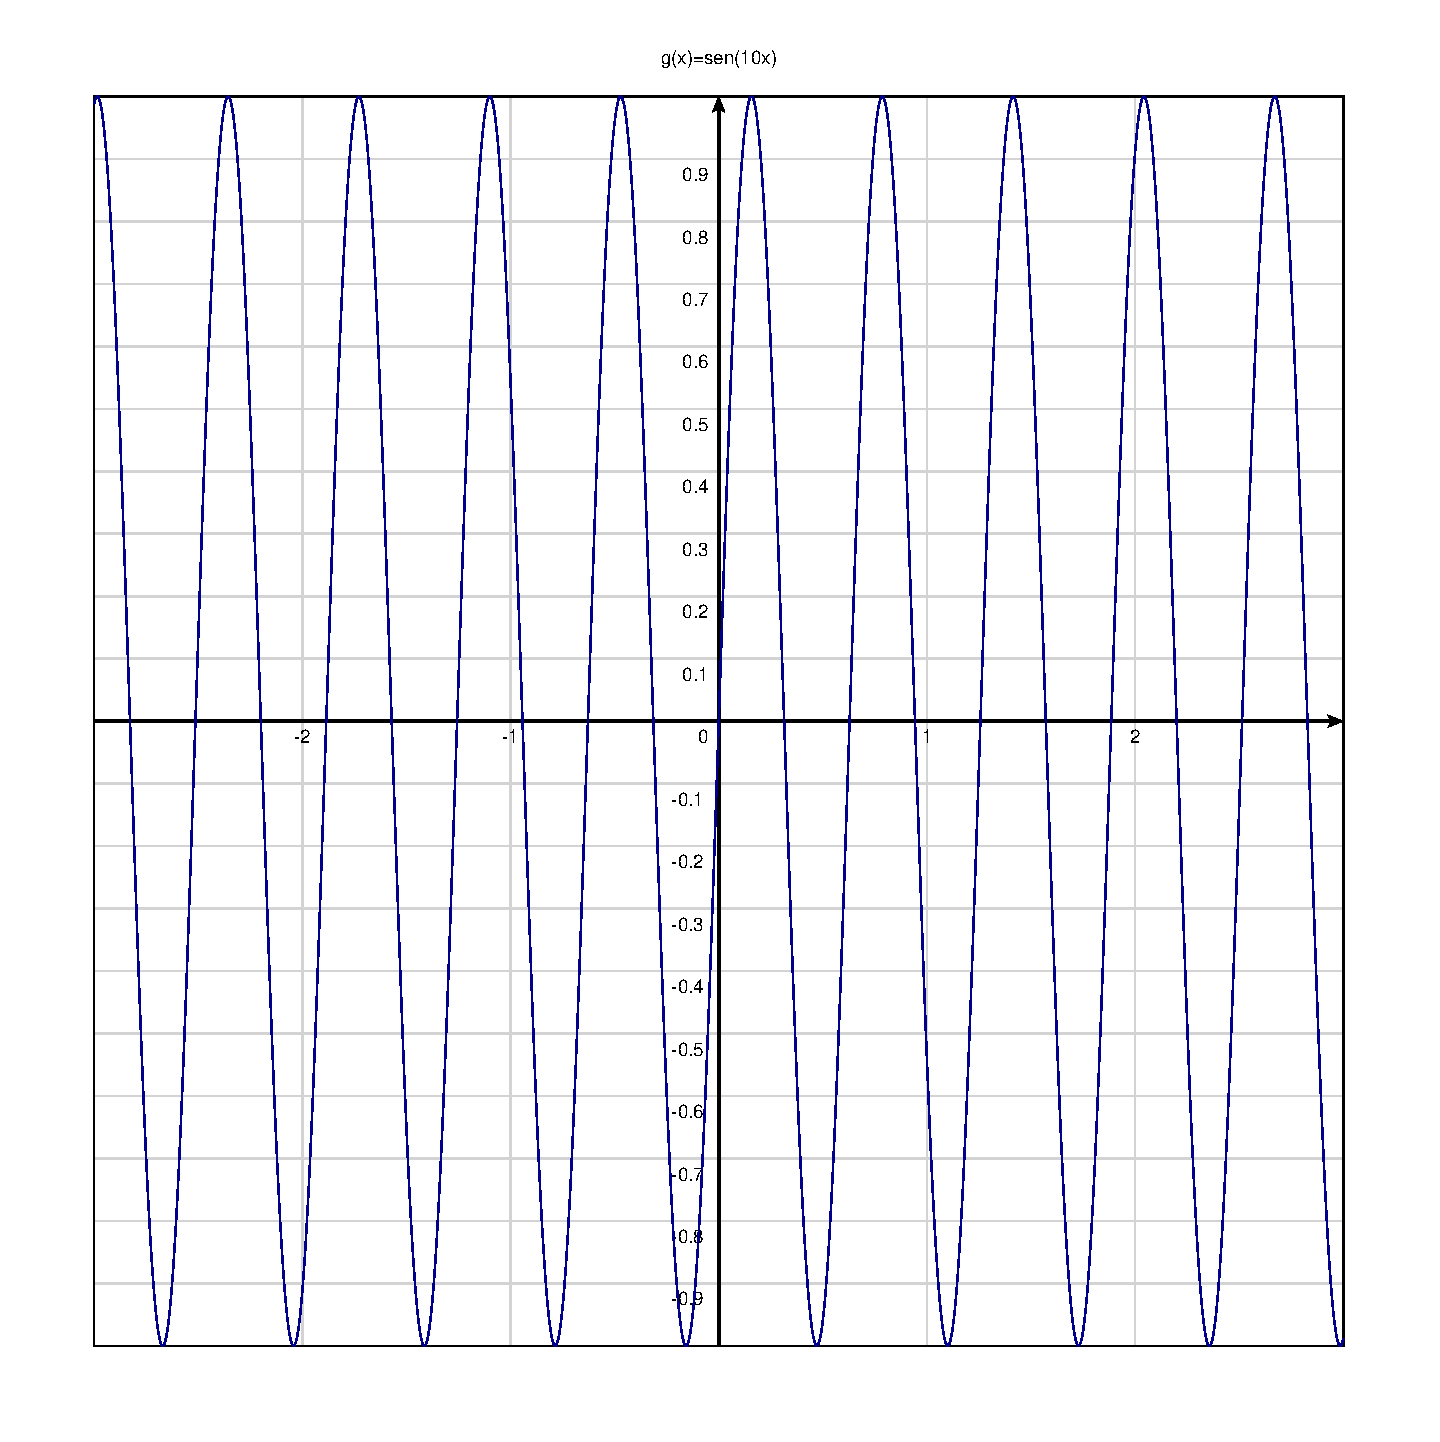
\includegraphics[width=\textwidth]{figures/graficaG.eps}
        \centering
        \caption{Gráfica de $h(x)$ evaluada en $[-3,3]$}
        \label{im:graficaG}
    \end{subfigure}
    \hfill
    \begin{subfigure}[b]{0.3\textwidth}
        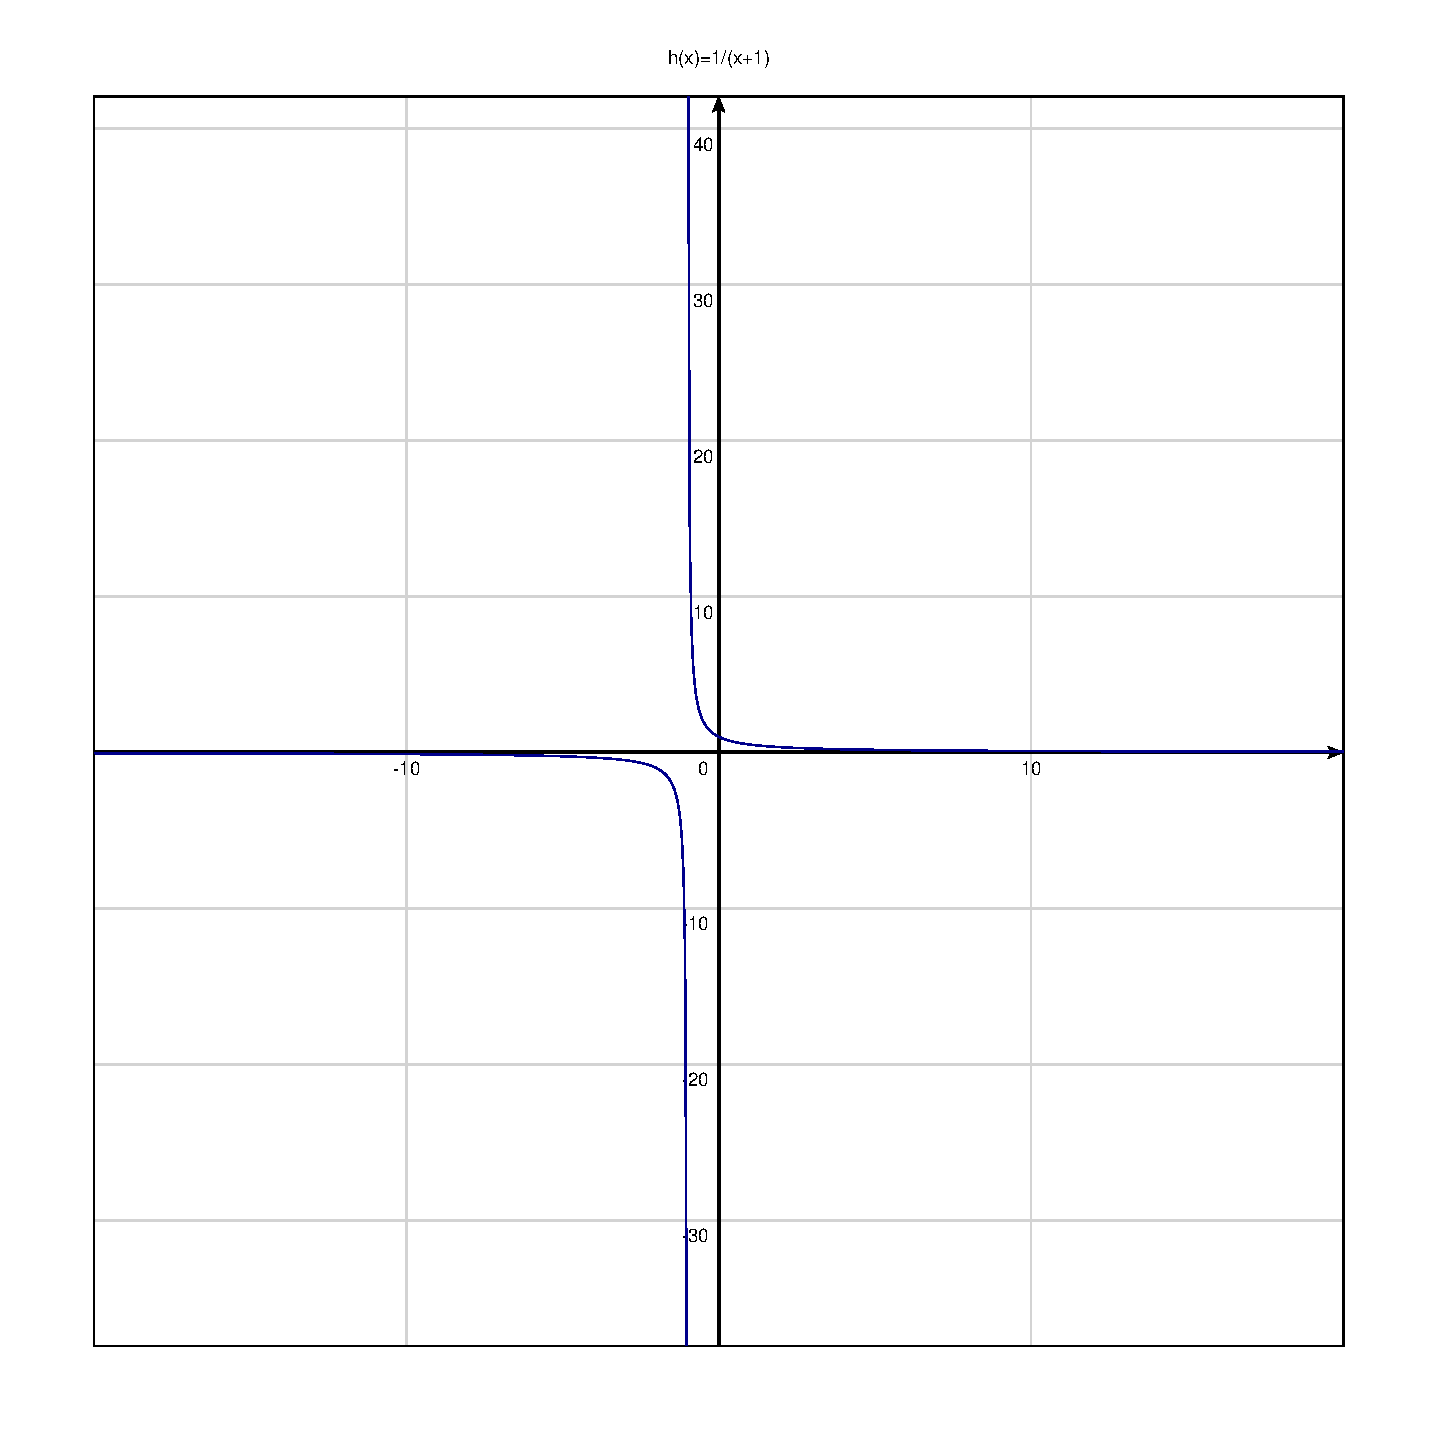
\includegraphics[width=\textwidth]{figures/graficaH.eps}
        \centering
        \caption{Gráfica de $h(x)$ evaluada en $[-20,20]$}
        \label{im:graficaH}
    \end{subfigure}
\end{figure}
\subsection{Problema 3}
En la figura \ref{im:zoom1} se muestra el zoom en la gráfica de $g(x)$ en el punto $x=0$, de forma que se muestra exactamente un ciclo de $g(x)$, es decir, evaluada en $\left[-\frac{\pi}{10},\frac{\pi}{10}\right]$. Más detalladamente, la figura \ref{im:zoom2} muestra el intervalo de $g(x)$ centrado en el punto $x=0$ en el que $g(x)$ es creciente, esto es, evaluada en $\left[-\frac{\pi}{20},\frac{\pi}{20}\right]$. Finalmente, la figura \ref{im:zoom3} muestra el zoom en la gráfica de $g(x)$ centrada en el punto $x=\frac{\pi}{20}$, de forma que se muestra la parte cóncava de un ciclo de $g(x)$, es decir, evaluada en $\left[0,\frac{\pi}{10}\right]$.
\begin{figure}[H]
    \begin{subfigure}[b]{0.3\textwidth}
        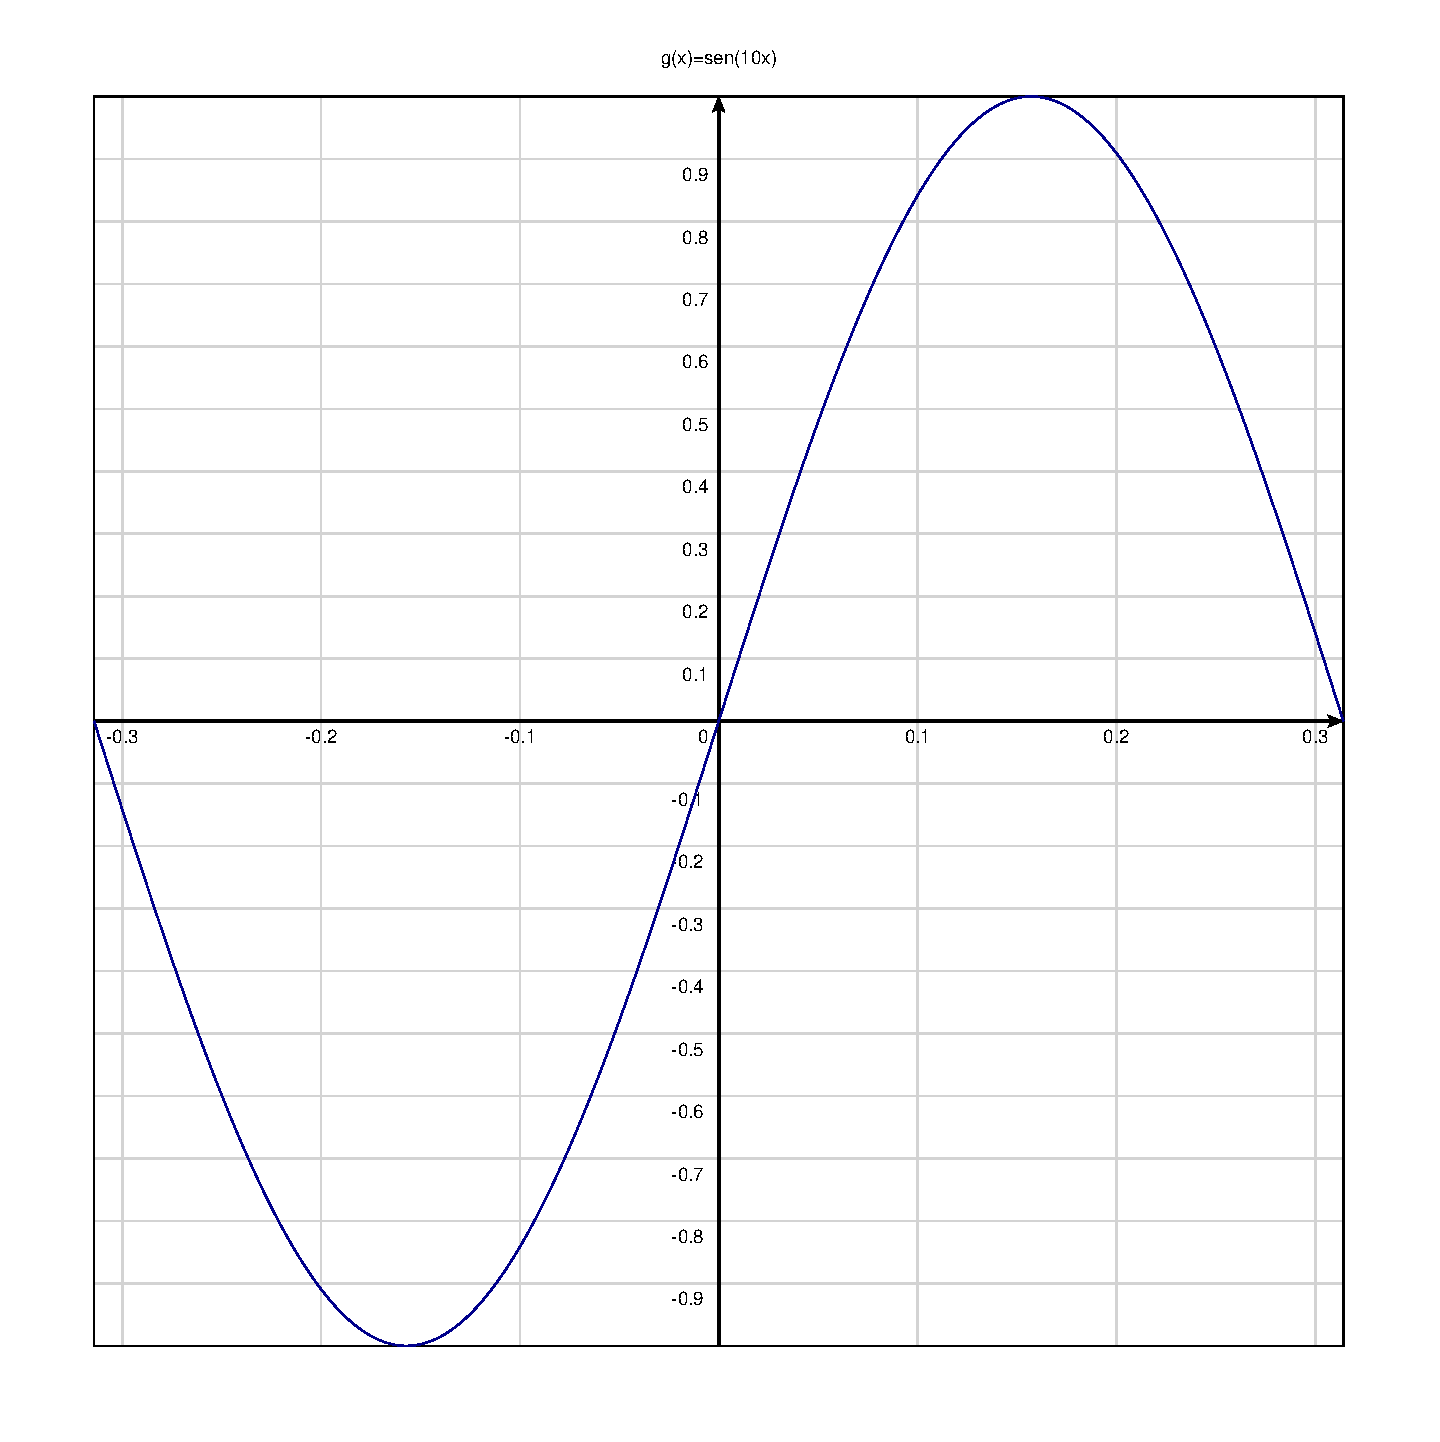
\includegraphics[width=\textwidth]{figures/Zoom1.eps}
        \centering
        \caption{Gráfica de $g(x)$ evaluada en $\left[-\frac{\pi}{10},\frac{\pi}{10}\right]$}
        \label{im:zoom1}
    \end{subfigure}
    \hfill
    \begin{subfigure}[b]{0.3\textwidth}
        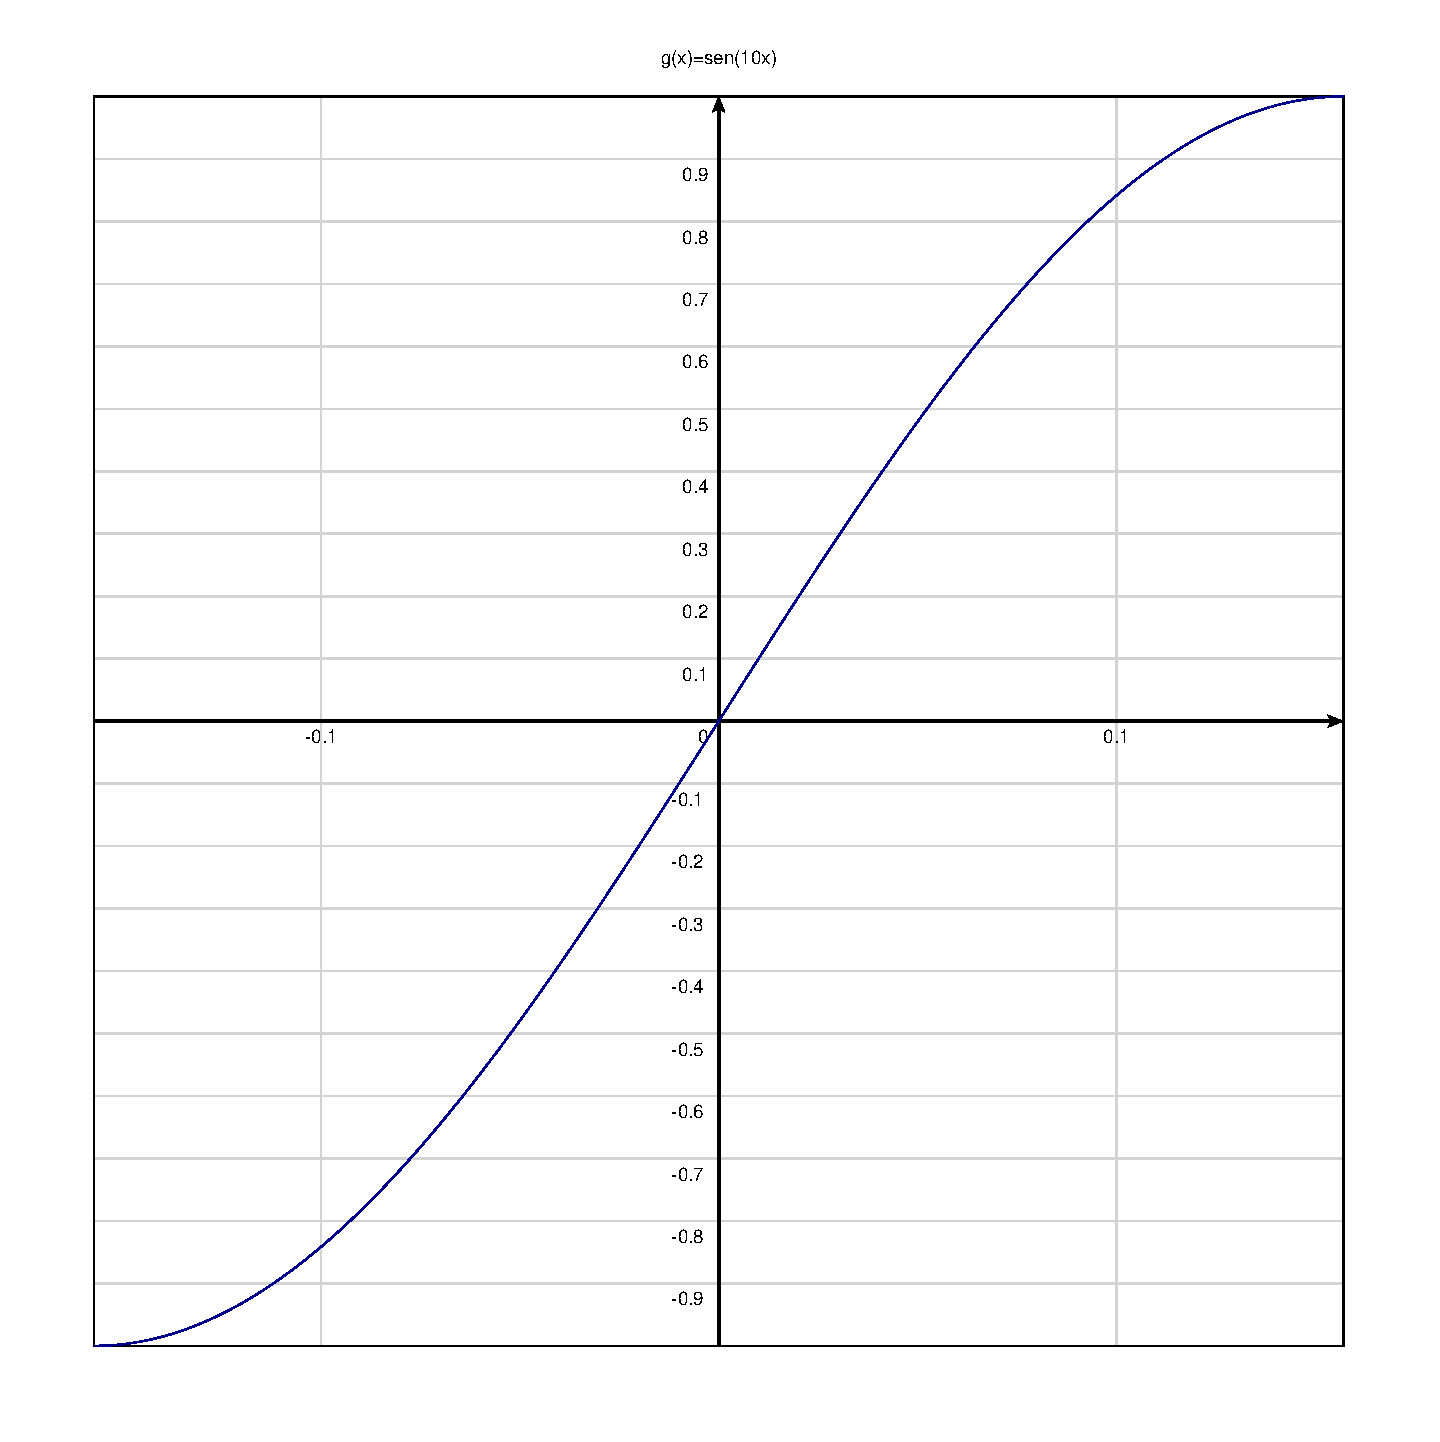
\includegraphics[width=\textwidth]{figures/Zoom2.eps}
        \centering
        \caption{Gráfica de $g(x)$ evaluada en $\left[-\frac{\pi}{20},\frac{\pi}{20}\right]$}
        \label{im:zoom2}
    \end{subfigure}
    \hfill
    \begin{subfigure}[b]{0.3\textwidth}
        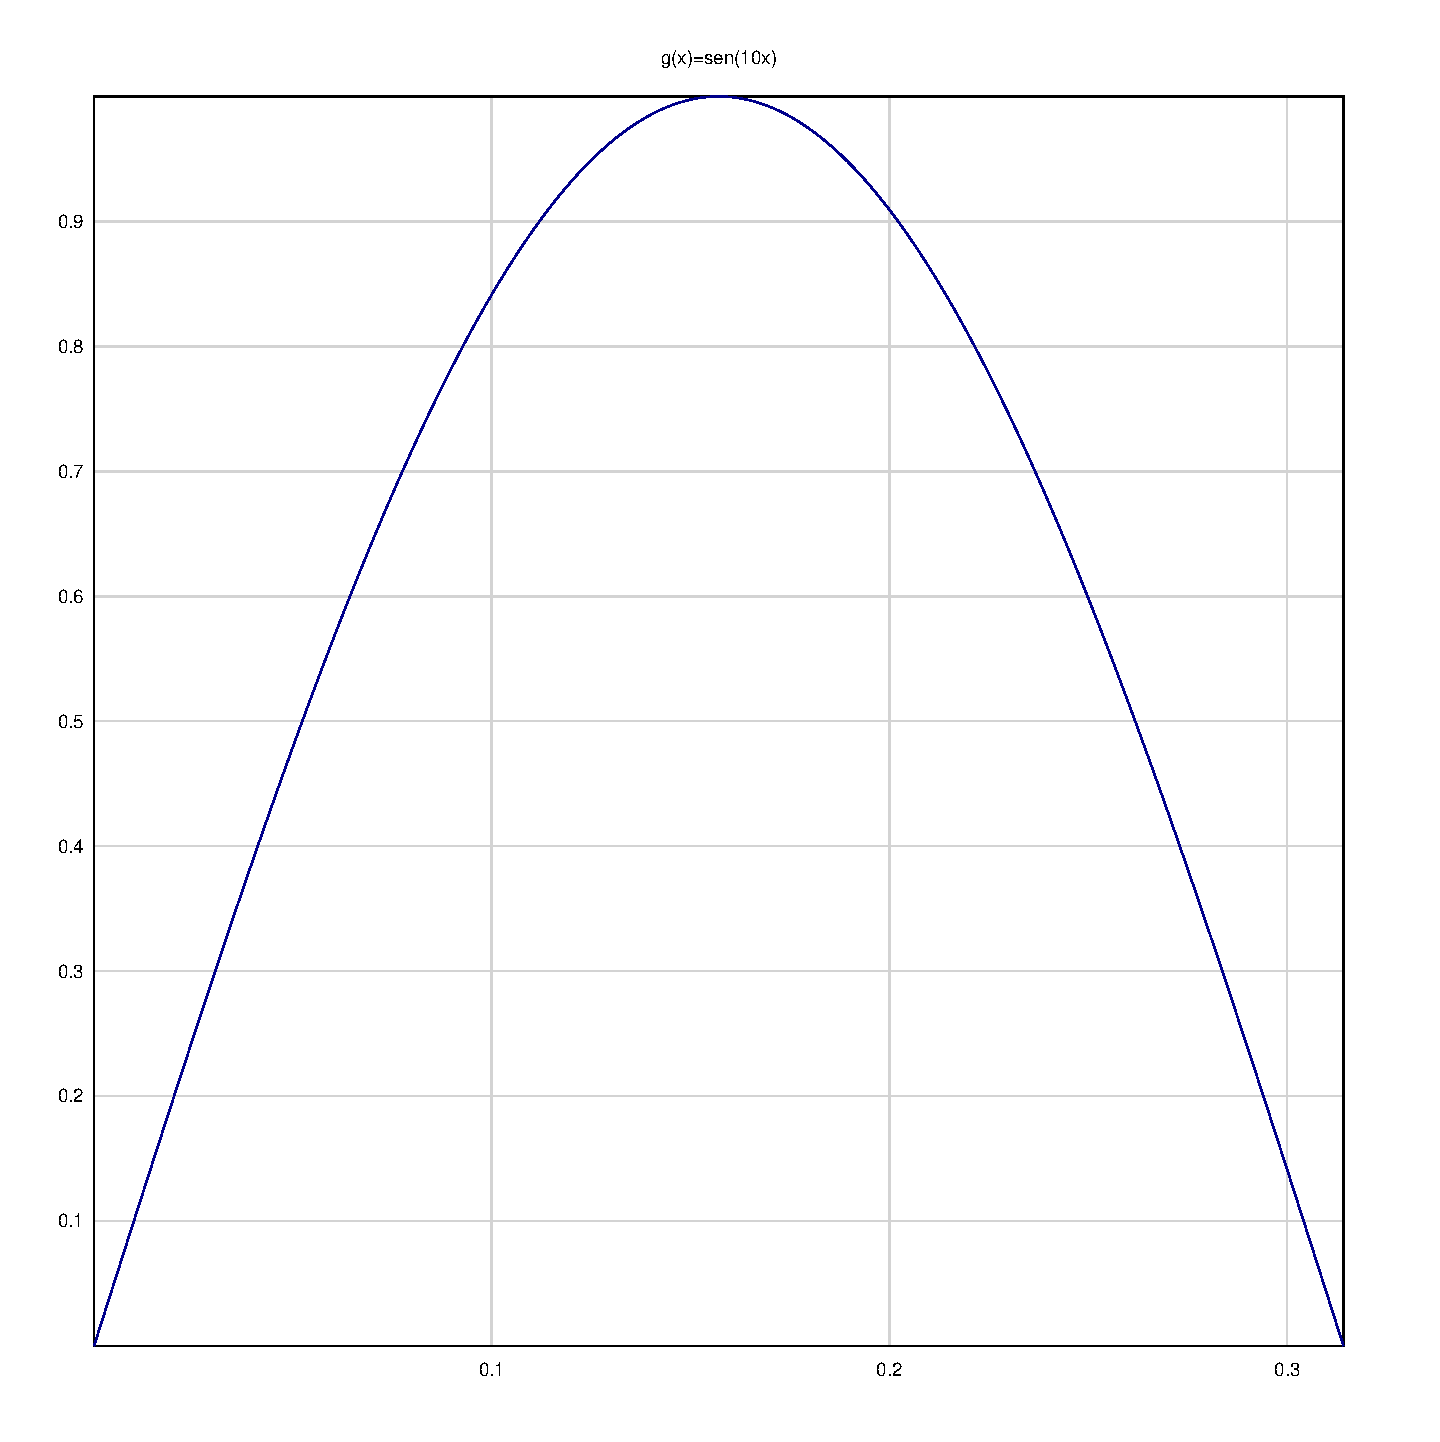
\includegraphics[width=\textwidth]{figures/Zoom3.eps}
        \centering
        \caption{Gráfica de $g(x)$ evaluada en $\left[0,\frac{\pi}{10}\right]$}
        \label{im:zoom3}
    \end{subfigure}
\end{figure}
\section{Conclusiones}
Un graficador es fundamental en el cálculo numérico, y nuestro graficador es suficiente para graficar funciones $f:\mathbb{R}\mapsto\mathbb{R}$ que podamos evaluar numéricamente, como lo vimos en esta tarea. La función de zoom lo hace más interesante, pues incluso otros graficadores muy utilizados no tienen esa característica.
\bibliography{biblio}
\bibliographystyle{elsarticle-num-names}
\end{document}
